\chapter{Structure fitting}

\section{Maximum filter: working principle}

In order to automatize completely this method, the introduction of additional layers for the image recognition are required. In Fig. \ref{fig:local_max} the different steps are shown:

\begin{itemize}
    \item First of all some features must be extracted from a given raw image i.e. the local maxima, that indicate where the spherical nanoparticles are located.
    \item This approach fails in understanding which local maxima are fit for our structure generation. For this reason, a threshold is introduced to choose which of the found points are valid. In this work the threshold has been set equal to the nominal radius of the nanoparticle.
\end{itemize}

\begin{figure}[ht]
    \centering
    % filtro_max
    \includegraphics[width=.95\textwidth]{./immagini/filtro_max.png}
    \caption{Steps for image recognition: a) Raw image b) Extracted local maxima c) Threshold application}
    \label{fig:local_max}
\end{figure}

\section{Tip size estimation}

Once the peaks have been found, we can obtain from their height the size of the nanoparticle we will be building. Once we have all the informations, we can generate the structure that will be used as a kernel for our morphological filter.

\begin{figure}[ht]
    \centering
    \begin{subfigure}[b]{0.325\textwidth}
        % 2_labl
        \includegraphics[width=.98\textwidth, trim={30, 0, 30, 0}, clip]{./immagini/2_labl.png}
        \caption{}
        \label{fig:process_steps_a}
    \end{subfigure}
    \hfill
    \begin{subfigure}[b]{0.325\textwidth}
        % 5_labl
        \includegraphics[width=.98\textwidth, trim={30, 0, 30, 0}, clip]{./immagini/5_labl.png}
        \caption{}
        \label{fig:process_steps_b}
    \end{subfigure}
    \hfill
    \begin{subfigure}[b]{0.325\textwidth}
        % 3_labl
        \includegraphics[width=.98\textwidth, trim={30, 0, 30, 0}, clip]{./immagini/3_labl.png}
        \caption{}
        \label{fig:process_steps_c}
    \end{subfigure}
    \caption{Process steps: a) Raw image b) Found peaks c) Generated structures}
    \label{fig:process_steps}
\end{figure}


Before reconstructing the tip, we need to estimate the domain/size of the tip, which can be done using the previous maps. It will ensure a good resolution and a low computing time. Once the structures have been fitted under the topography, the tip matrix size must be estimated to cover the largest sample present in the image. However, in order to have an high resolution tip after the erosion process, it is important not to overestimate this parameter. In fact, the size of the convolution output matrix is determined by the difference in the number of pixels between the structure size and the original data size. Also the underestimating of the tip matrix size would be an issue, since the result would include only the tip apex with loss of tip sides.

To estimate the largest feature in the sample we approach the problem by creating a mask (Fig. \ref{fig:boolean_a}) able to select only the points with the height values greater than a given threshold. Therefore, to obtain the perimeter of the areas, the derivative calculation of the boolean mask is performed along X and Y direction (Fig. \ref{fig:boolean_b}).

\newpage

\begin{figure}[ht]
    \centering
    \begin{subfigure}[b]{0.45\textwidth}
        % maschera_picchi
        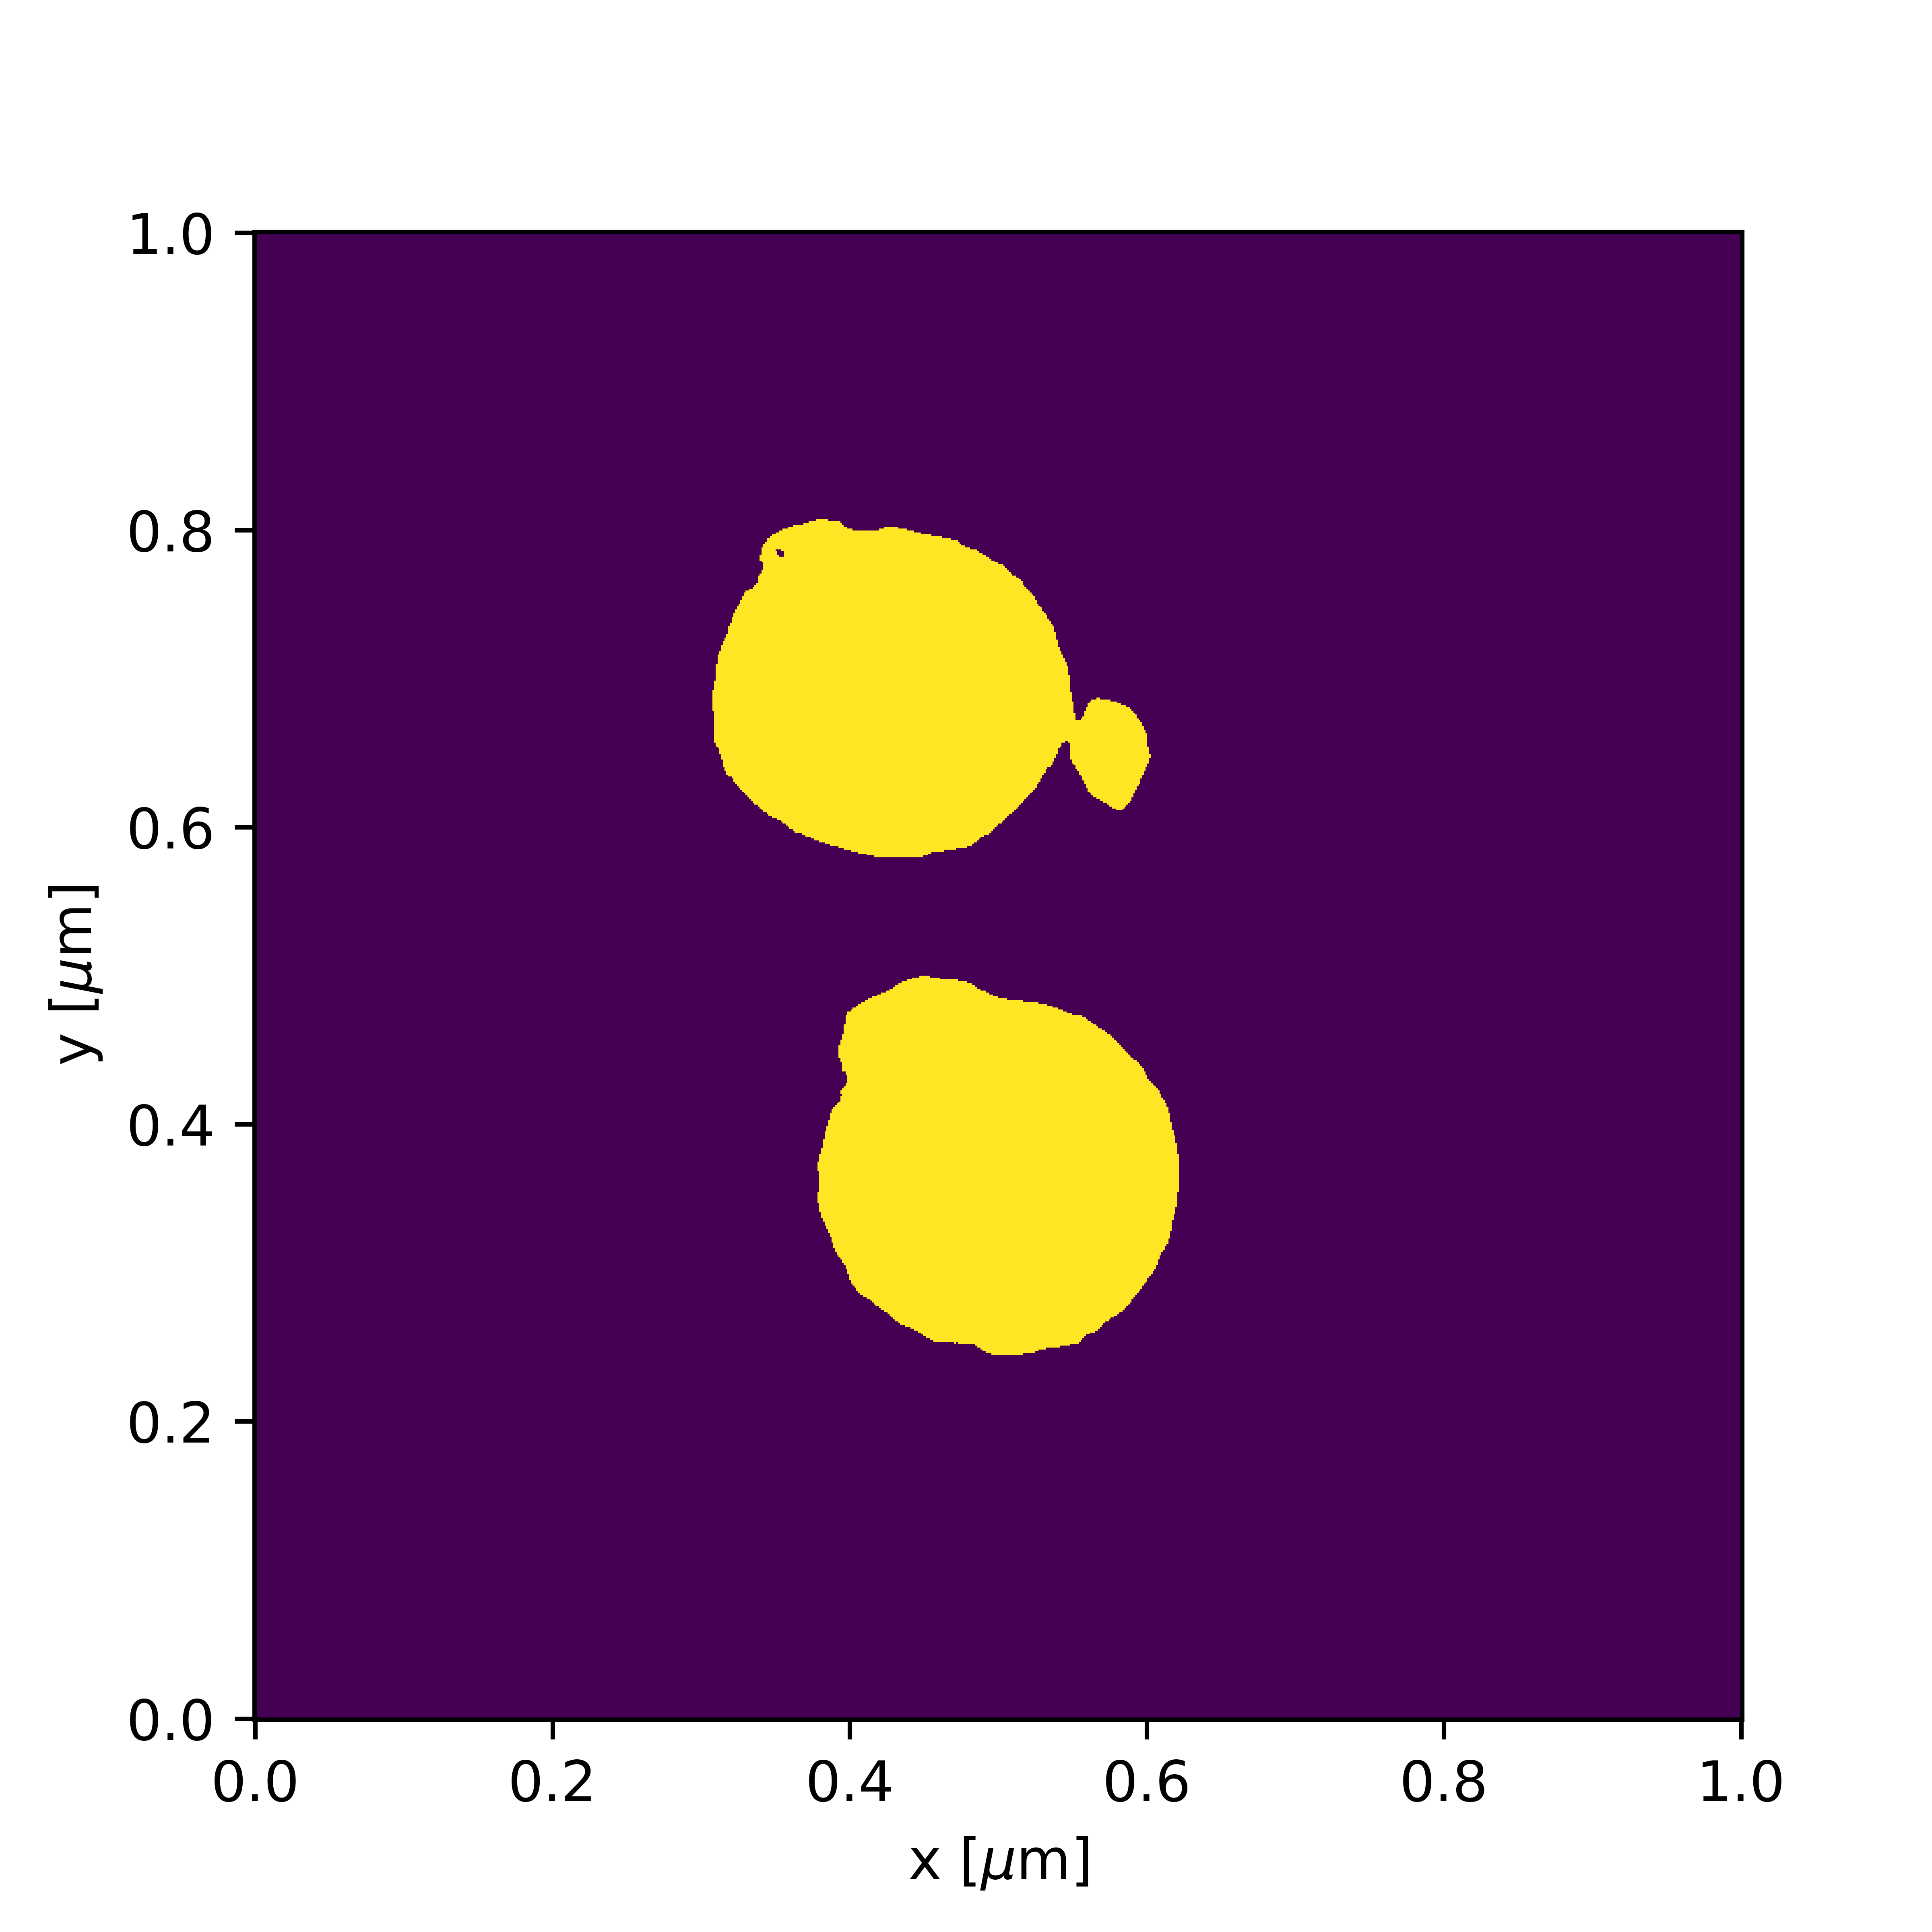
\includegraphics[width=.98\textwidth]{./immagini/maschera_picchi.png}
        \caption{}
        \label{fig:boolean_a}
    \end{subfigure}
    \hfill
    \begin{subfigure}[b]{0.45\textwidth}
        % derivatives
        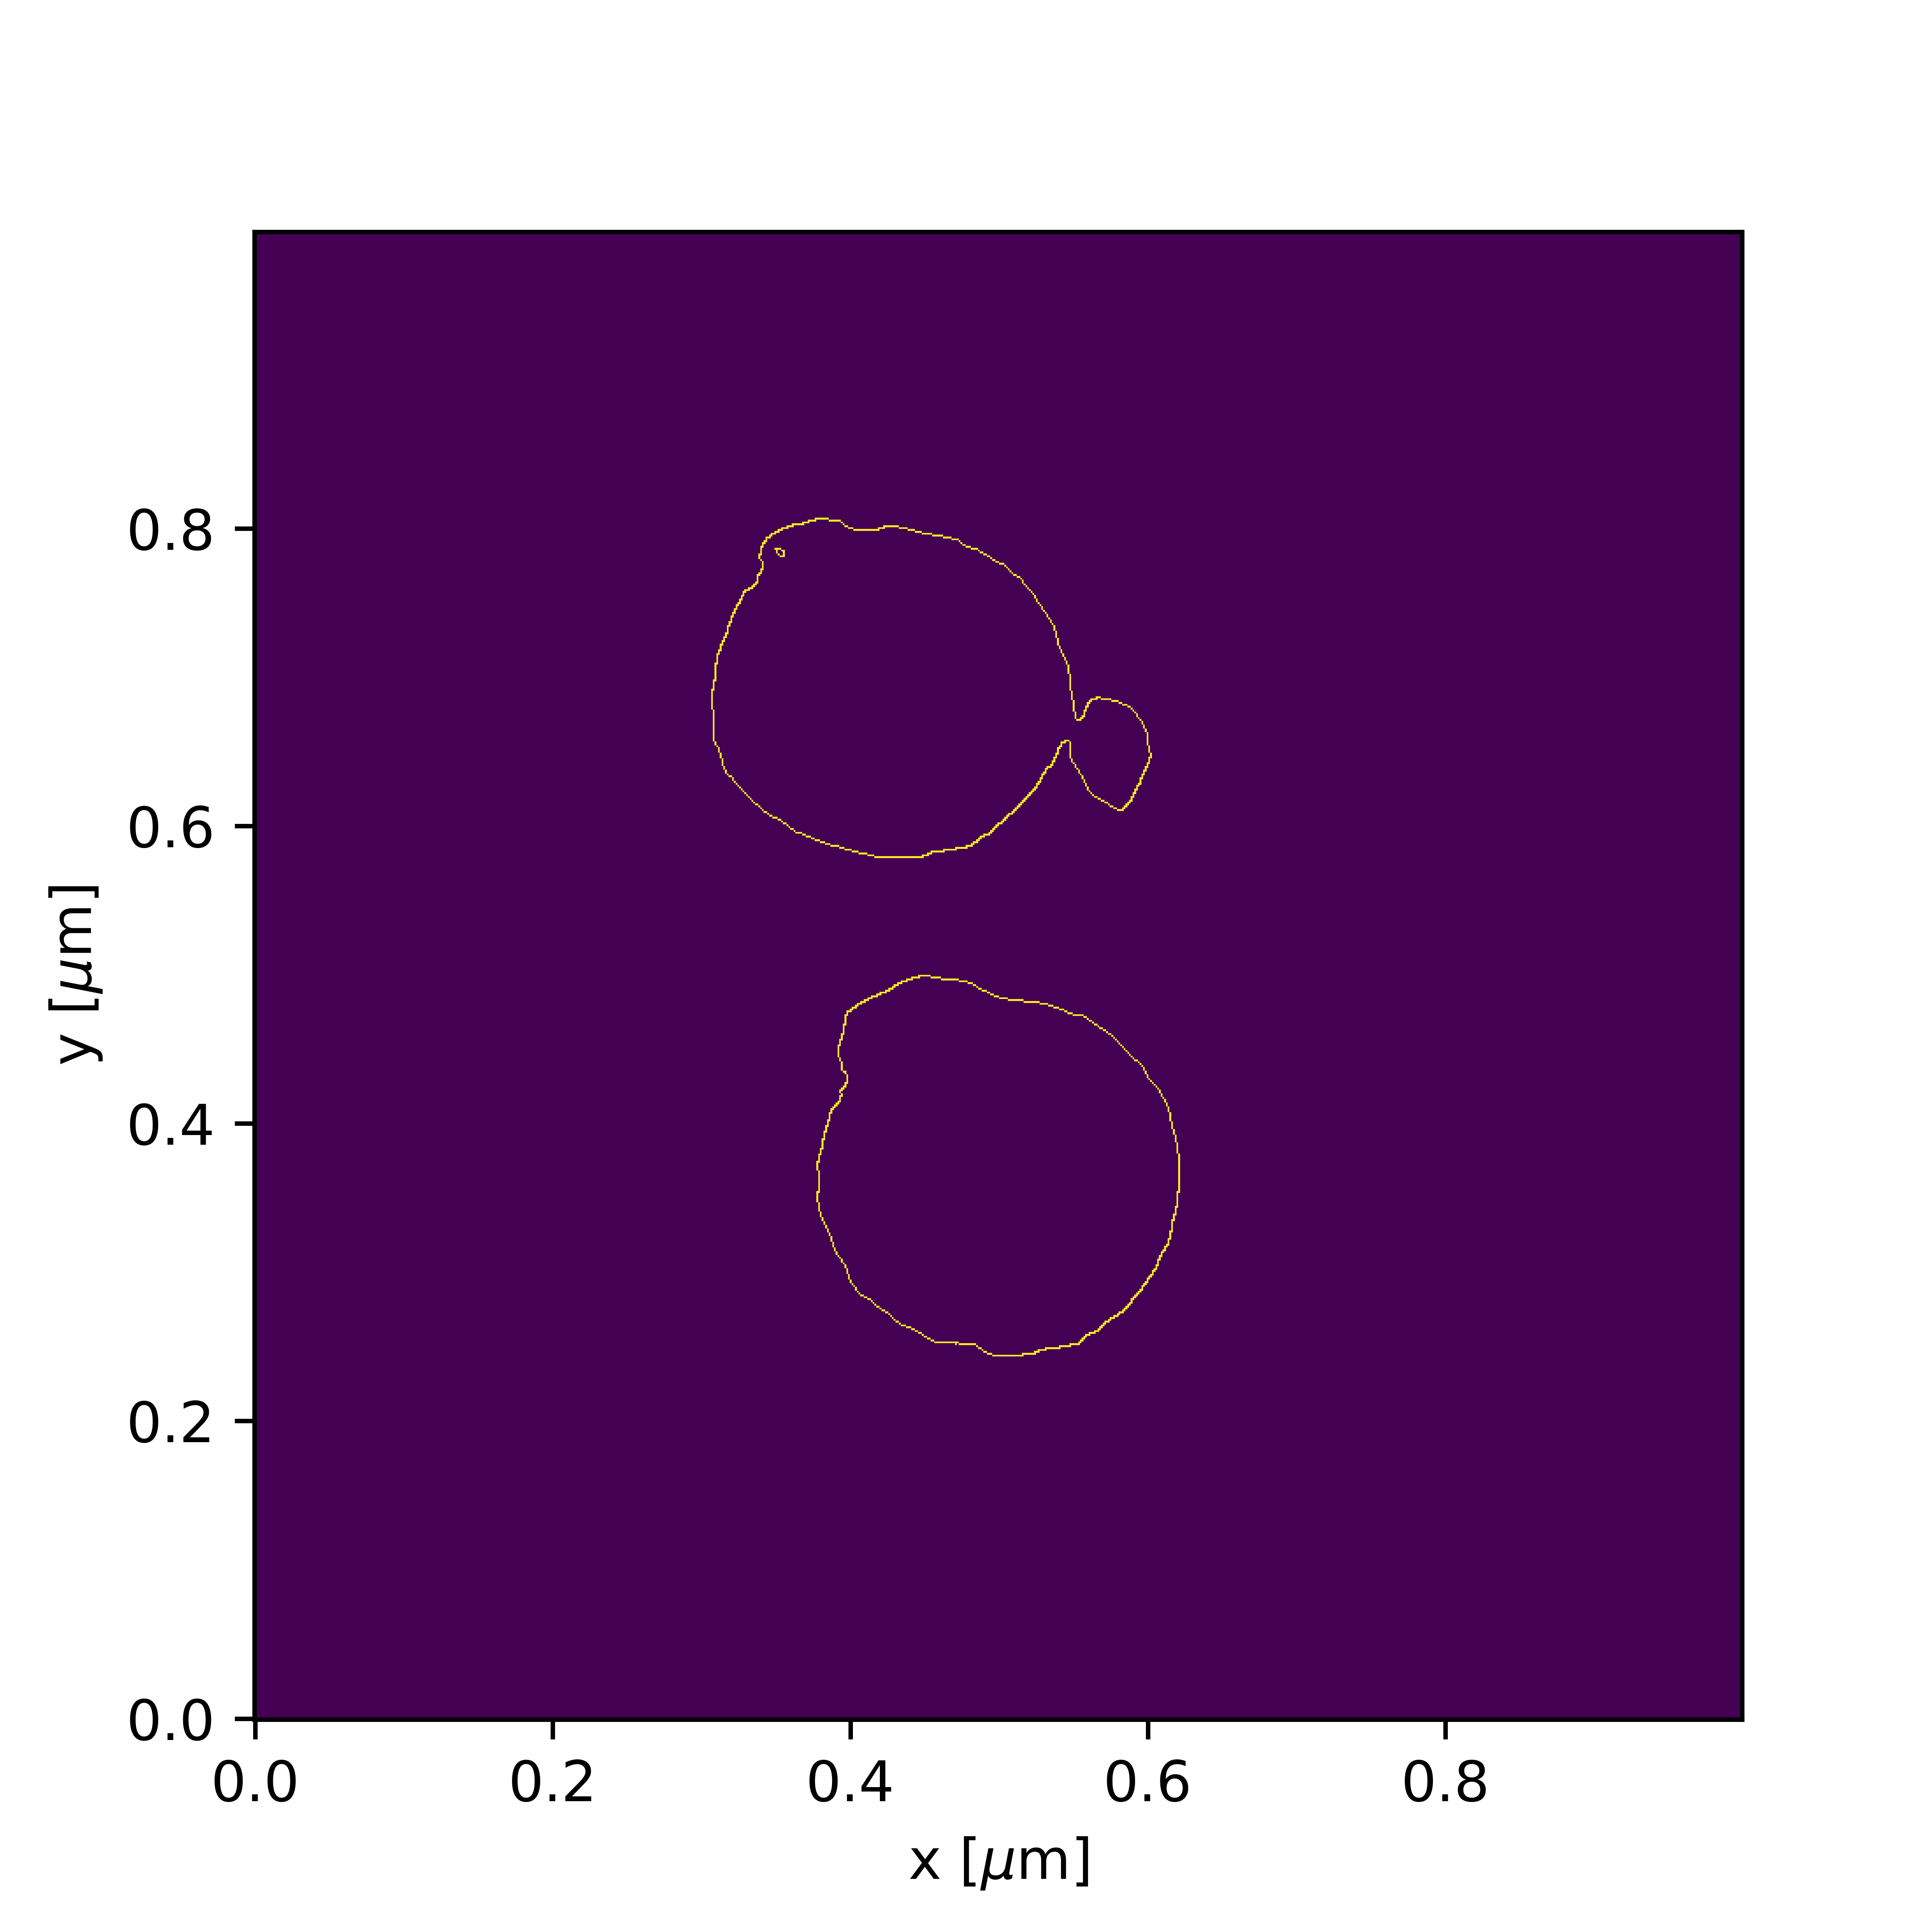
\includegraphics[width=.98\textwidth]{./immagini/derivatives.png}
        \caption{}
        \label{fig:boolean_b}
    \end{subfigure}
    \caption{a) mask, b)  binary derivation for Tip size estimation}
    \label{fig:boolean}
\end{figure}

It is known that the derivative of a boolean mask returns True if there's a change in the value of the data and False otherwise. Then, we scan line by line each in both directions and all the extracted True indices have been coupled. The difference of the elements in each couple represents the width of the feature between the two indices. The maximum value of this difference was finally used as a parameter to obtain the final tip matrix size, which will be increased by an additional radius (example: +10\%) to guarantee a border around the reconstructed tip.